\begin{figure}[htbp]
    \caption{Impact of Departures on Organizational Outcomes}
    \label{fig:prs_opened}
    \centering
    \begin{minipage}[b]{0.49\textwidth}
        \centering
        \subcaption{All organizations} \label{fig:all_prs_opened}
        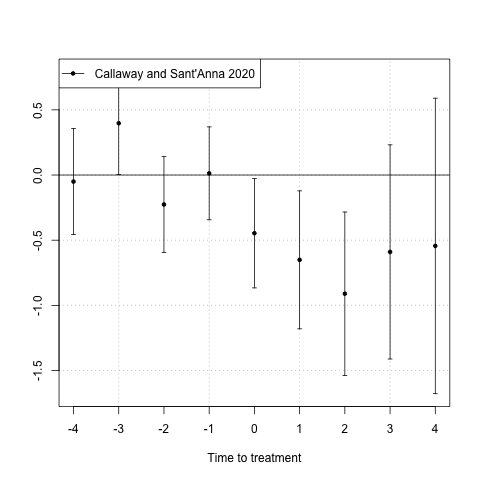
\includegraphics[width=\textwidth]{temp/output/prs_opened_norm.png}
    \end{minipage}
    \hfill
    \begin{minipage}[b]{0.49\textwidth}
        \centering
        \subcaption{By collaborativeness}\label{fig:all_prs_opened_collab}
        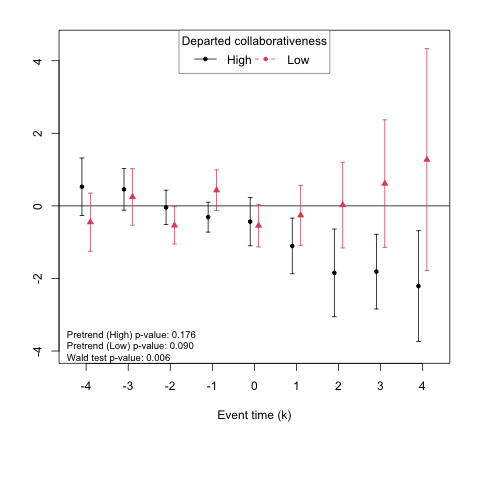
\includegraphics[width=\textwidth]{temp/output/collab/prs_opened_collab_cs_norm.png}
    \end{minipage}
  \vspace{1ex}
  \centering
  \begin{minipage}{1\textwidth}
    \textbf{Figure notes:} 
    Following Callaway and Sant’Anna (2021), I estimate event-study coefficients accompanied by 95\% simultaneous confidence bands. For each plot with event study estimates from two subsamples, I report three Wald-test p-values: one for the pretrend test in the first subsample, one for the pretrend test in the second subsample (both from Equation \ref{eq:wald_test_pretrends} in Section \ref{sec:main_method}), and one for the difference in treatment effects across subsamples (Equation \ref{eq:wald_test} in Section \ref{sec:att_subset}). Panel~\subref{fig:all_prs_opened} plots event study estimates that use the full set of projects. Panel~\subref{fig:all_prs_opened_collab} plots two sets of event study estimates: projects with highly collaborative departed contributors and projects with less collaborative departed contributors. In all panels, the outcome is the pull request z score, transformed using the pre-treatment mean and standard deviation.
  \end{minipage}


\end{figure}
